\chapter{Achtergrond}

\section{Displacement pipetten}
Hoewel er diverse pipetprincipes bestaan, zoals volumetrische glazen pipetten (bijvoorbeeld buretten) en gravimetrische dispensers, richt dit werk zich uitsluitend op displacement pipetten. Deze categorie is het meest relevant voor geautomatiseerde vloeistofhanteringssystemen doordat ze eenvoudig te integreren zijn in robotica en een breed scala aan vloeistoffen kunnen verwerken.

\subsection{Air displacement}
Bij air-displacement pipetten is er geen direct contact tussen de zuiger en de vloeistof; een luchtlaag scheidt beide. Dit voorkomt contaminatie, wat een belangrijk voordeel is. De keerzijde is een lagere nauwkeurigheid, veroorzaakt door luchtdrukschommelingen en oppervlaktespanning in de vloeistof.
\\[12pt]Deze fouten kunnen deels gecorrigeerd worden met berekeningen, zoals beschreven in het werk van T. W. Astle et al.\ \cite{RN15}, of met lookup-tabellen van Nelson et al.\ \cite{RN35}, maar dit werkt niet altijd. Vooral bij zeer kleine volumes is de invloed van oppervlaktespanning zo groot dat correctie onmogelijk wordt. In zulke gevallen biedt positive displacement, zoals eveneens beschreven door Astle\ \cite{RN15}, een oplossing.

\subsubsection{Theoretische achtergrond}
In het werk van T. W. Astle et al.\ \cite{RN15} staat beschreven hoe een air-displacement pipet werkt via de ideale gaswet. Er wordt een omgeving van lagere druk gecreëerd door het veranderen van het volume van de pipet. Dit volume wordt ingenomen door de vloeistof waar de pipetpunt zich in bevindt. Bij een mondpipet wordt deze negatieve druk gecreëerd door de longen van de operator. Bij de mechanische pipet wordt deze via de peer gecreëerd door deze initieel in te drukken en daarna terug te laten opvullen.

\subsection{Positive displacement}
Positive displacement pipetten zijn een alternatieve oplossing waarbij er wel contact is tussen de vloeistof en de zuiger. Er treden dus geen oppervlaktespanningen op aangezien de vloeistof overal contact maakt met de zuiger. Dit heeft voordelen op vlak van precisie, vooral bij vloeistoffen die sterk verschillen van water. Zo worden positive displacement pipetten in het werk van Henke en Eppendorf\ \cite{RN37} voorgesteld als methode om cel-cultuur-media of BSA te pipetteren. Ze dragen echter een groter risico op contaminatie, al kan dit wel voorkomen worden door bijvoorbeeld het gebruik van verwisselbare pipettips.

\section{Pipet types}
\subsection{Analoge pipetten}\label{sec: Analoge pipetten}
Analoge pipetten werken met een zuigermechanisme, waarbij het volume wordt ingesteld door de slag van de zuiger aan te passen. In het werk van Al-Mahareeq en Al-Mahrouq Hasan\ \cite{RN17} (zie \autoref{fig:werking US5320810}) gebeurt dit via een instelwiel dat de zuigerstang verplaatst, waardoor het volume verandert. Bij Shapiro\ \cite{RN16} (zie \autoref{fig:werking US4744955}) wordt het volume ingesteld door het ondergedeelte van de pipet in te schroeven, wat de zuigerpositie en slag aanpast.

\begin{minipage}[t]{0.49\textwidth}
    \vspace{0pt}
    \begin{figure}[H]
        \centering
        \captionsetup{width=0.85\textwidth}
        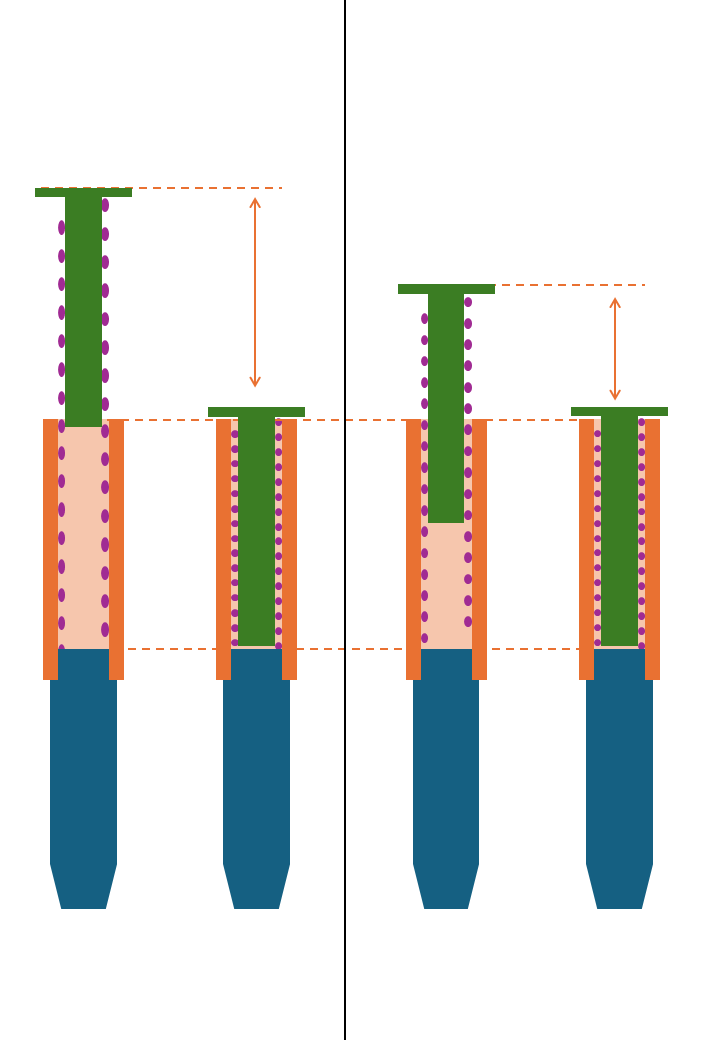
\includegraphics[width=0.49\textwidth]{figures/Werking US5320810.png}
        \caption{Werking van de analoge pipet beschreven in US5320810, waar de beginpositie van de zuiger ingesteld wordt.}\label{fig:werking US5320810}
    \end{figure}
\end{minipage}
\begin{minipage}[t]{0.49\textwidth}
    \vspace{0pt}
    \begin{figure}[H]
        \centering
        \captionsetup{width=0.85\textwidth}
        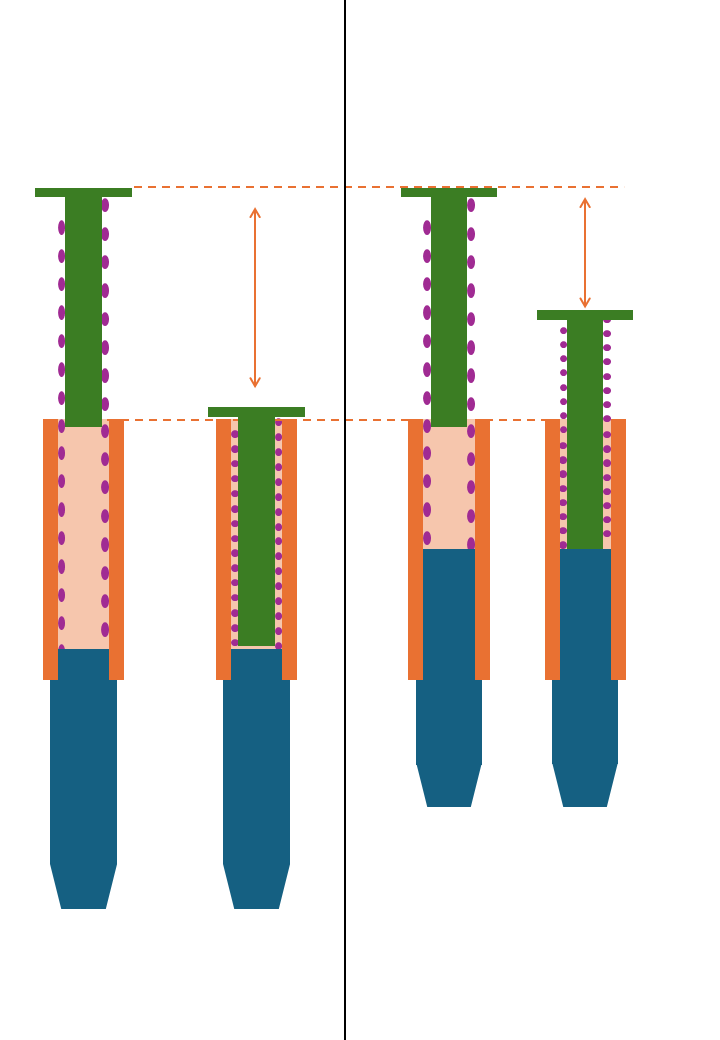
\includegraphics[width=0.49\textwidth]{figures/Werking US4744955.png}
        \caption{Werking van de analoge pipet beschreven in US4744955, waar de eindpositie van de zuiger ingesteld wordt.}\label{fig:werking US4744955}
    \end{figure}
\end{minipage}
\\[12pt]De pipetten gebruiken meestal air-displacement, maar er zijn ook varianten met positieve displacement. De pipetten beschreven door Shapiro\ \cite{RN16} zijn eenvoudiger, maar kunnen meer lekkage en onnauwkeurigheid vertonen dan de uitvoering van Al-Mahareeq en Al-Mahrouq Hasan\ \cite{RN17}.

\subsection{Elektronische pipetten}
Elektronische pipetten gebruiken motoren (vaak met een loodschroef) zoals stappermotoren om de zuiger nauwkeurig te verplaatsen. Nelson et al.\ \cite{RN35} passen microstepping toe om de beweging te verfijnen, wat een nauwkeurigheid van enkele nanoliters mogelijk maakt. Het systeem kan verder worden geoptimaliseerd met een lookup- en calibratietabel. Problemen kunnen optreden bij gemiste stappen, wat leidt tot volumefouten. In een closed-loop systeem, zoals beschreven door Lind en Pekkanen\ \cite{RN36}, wordt een sensor gebruikt om deze fouten te corrigeren.

\section{Bestaande liquid handling robots}
Voor geautomatiseerd pipetteren bestaan zowel commerciële systemen als open source alternatieven. In dit hoofdstuk worden beide categorieën besproken, met aandacht voor hun werking, kosten en geschiktheid voor verschillende toepassingen.
\subsection{Commerciële oplossingen (closed source)}
Commerciële systemen zoals Andrew+ en Opentrons OT-2 zijn populaire keuzes in laboratoria. De Andrew+ (\autoref{fig:Andrew}) biedt geavanceerde functionaliteit en is modulair, maar heeft een gesloten softwareomgeving. De Opentrons OT-2 (\autoref{fig:OT2}) is betaalbaarder, maar is ook gesloten wat betreft hardware- en software-aanpassingen. Beide systemen zijn gebruiksvriendelijk, maar hun gesloten aard en hoge kosten maken ze minder geschikt als goedkope open-source oplossing.
\\[12pt]
\begin{minipage}[t]{0.49\textwidth}
    \vspace{0pt}
    \begin{figure}[H]
        \centering
        \captionsetup{width=0.85\textwidth}
        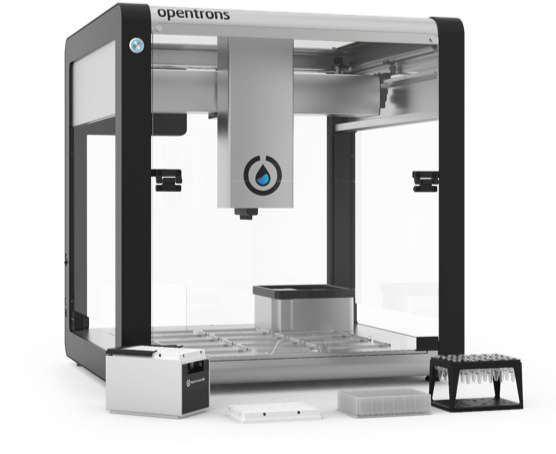
\includegraphics[height=2.5cm]{figures/opentronsot2.png}
        \caption{Opentrons OT-2}\label{fig:OT2}
        \textbf{Prijs}: \$15'000+\\
        \textbf{Bron}: Opentrons\ \cite{RN27}
    \end{figure}
\end{minipage}
\begin{minipage}[t]{0.49\textwidth}
    \vspace{0pt}
    \begin{figure}[H]
        \centering
        \captionsetup{width=0.85\textwidth}
        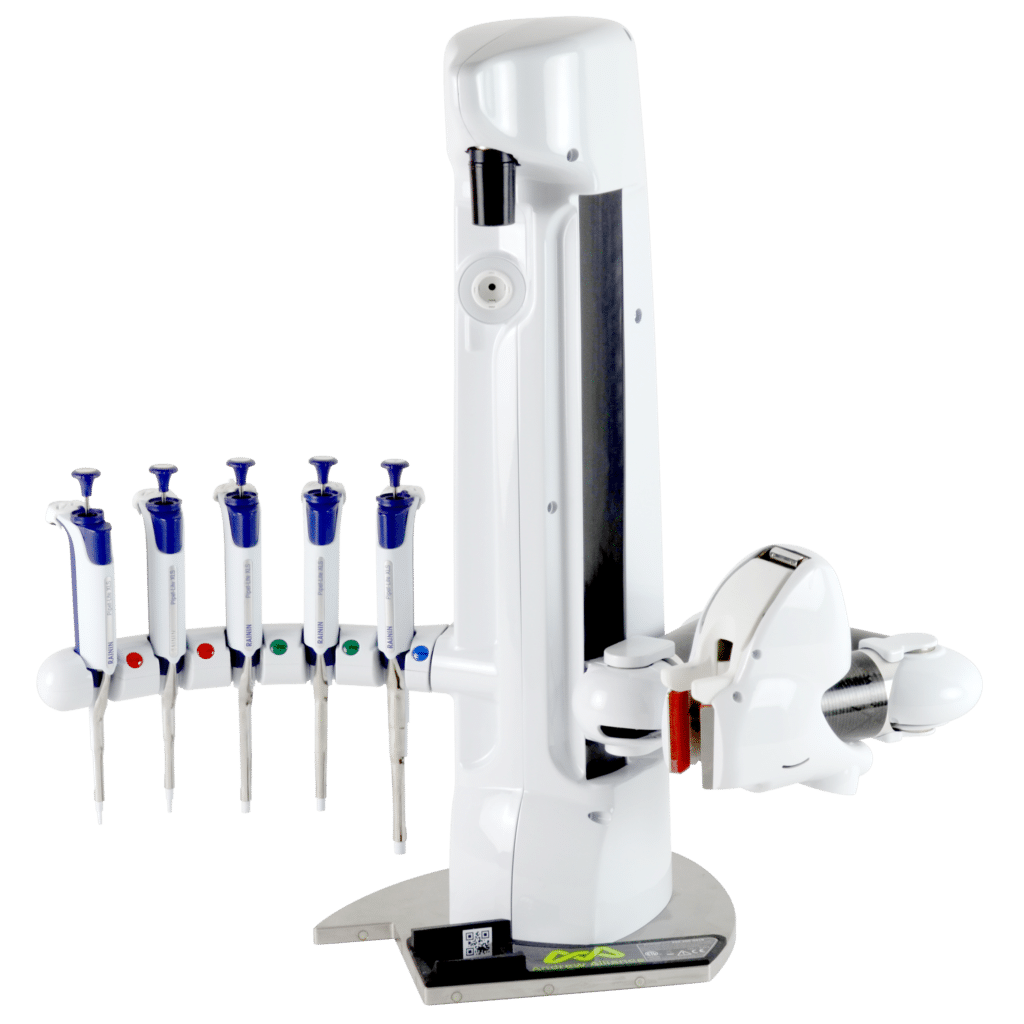
\includegraphics[height=2.5cm]{figures/Andrew-Alliance-liquid-handling-robot.png}
        \caption{Andrew Alliance Andrew+}\label{fig:Andrew}
        \textbf{Prijs}: \$20'000+ \\ 
        \textbf{Bron}: Andrew Alliance\ \cite{RN28}
    \end{figure}
\end{minipage}

\subsection{Open source oplossingen}
Open source oplossingen maken pipetteren toegankelijker voor kleinere instellingen. Twee voorbeelden zijn de robot van Kopyl et al. (2024)\ \cite{RN42} en de Sidekick van Keesey et al. (2022)\ \cite{RN41}.

\subsubsection{Sidekick (Keesey et al.)}
De Sidekick\ \cite{RN41} is een 3D-geprinte robot met vier solenoïde-gedreven micropompen voor positive displacement. De robot wordt aangestuurd door een Raspberry Pi Pico en kan via eenvoudige tekstcommando’s of beperkte G-code worden bediend. De kosten bedragen ongeveer \$710.
\\[12pt]De end effector bestaat uit vier vaste uitgangen (P1–P4), elk verbonden met een micropomp. Er is geen bewegende zuiger of pipet; vloeistof wordt rechtstreeks vanuit een reservoir gepompt via PTFE-slangen naar het gewenste doel. Omdat enkel gedispenseerd wordt (zonder aspiratie), is deze setup vooral geschikt voor toepassingen zoals reagentia-distributie. Door het ontbreken van z-as-bewegingen is de mechanische complexiteit sterk gereduceerd.

\subsubsection{3D-printer-gebaseerde oplossing (Kopyl et al.)}
Kopyl et al.\ \cite{RN42} ontwikkelden een pipetteerrobot op basis van een Creality Ender 3 Pro 3D-printer. De pipet wordt aangedreven door een stappermotor via een ball screw, en kan zowel air- als positive displacement pipetten bedienen. Het systeem is goedkoop (ca. \$325) en gebruikt open-loop controle zonder detectie van de pipetstand. Het te pipetteren volume moet door de gebruiker manueel worden ingesteld. In het ontwerp van deze thesis daarentegen wordt het volume door een motor bepaald en kan de pipet volledig autonoom werken.
\\[12pt]\begin{minipage}[t]{0.49\textwidth}
    \vspace{0pt}
    \begin{figure}[H]
        \centering
        \captionsetup{width=0.85\textwidth}
        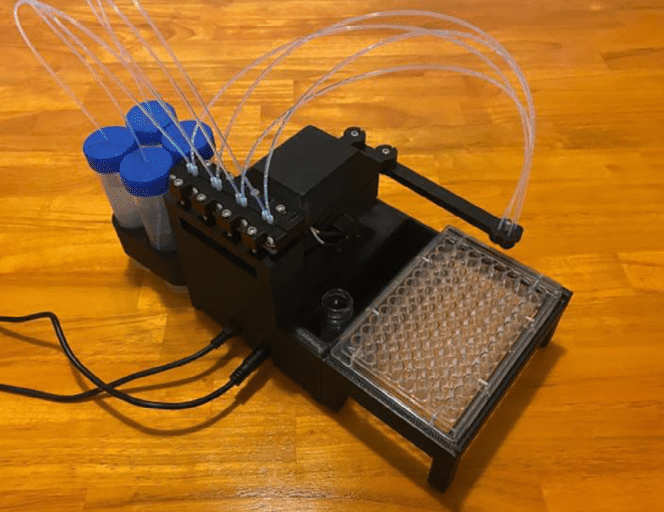
\includegraphics[height=2.5cm]{figures/Sidekick.png}
        \caption{Sidekick}\label{fig:Sidekick}
        \textbf{Prijs}: \$710\\
        \textbf{Bron}: Keesey et al.\ \cite{RN41}
    \end{figure}
\end{minipage}
\begin{minipage}[t]{0.49\textwidth}
    \vspace{0pt}
    \begin{figure}[H]
        \centering
        \captionsetup{width=1\textwidth}
        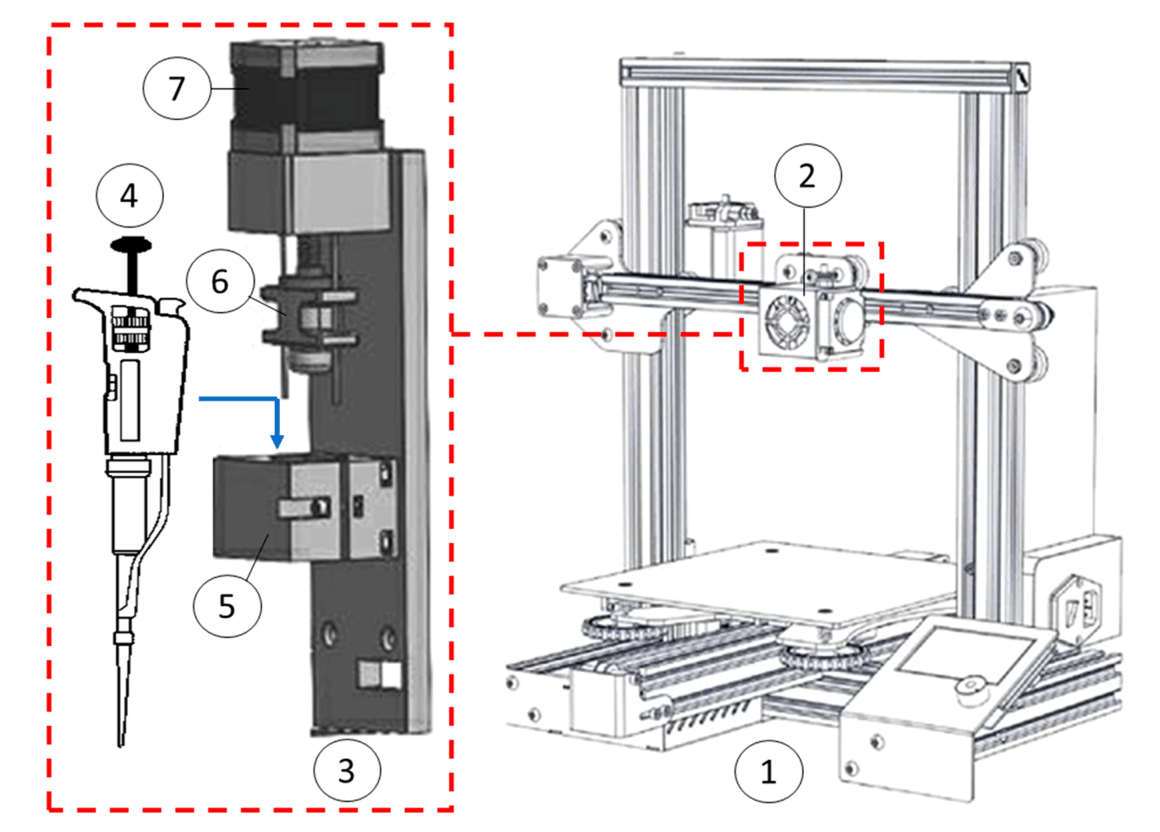
\includegraphics[height=2.5cm]{figures/kopyl-et-al.png}
        \caption{Kopyl et al.}\label{fig:kopyl}
        \textbf{Prijs}: \$325\\
        \textbf{Bron}: Kopyl et al.\ \cite{RN42}
    \end{figure}
\end{minipage}
